\documentclass[12pt,a4paper]{article}
\usepackage[utf8]{inputenc}
\usepackage{graphicx}
\usepackage{caption}
\usepackage{subcaption}
\usepackage{amsmath}
\usepackage{geometry}
\geometry{margin=1in}
\usepackage{booktabs}
\usepackage{hyperref}
\usepackage{float}

\title{\textbf{Credit Card Behaviour Score Prediction}}
\author{
    Utsah \\ 
    Enrollment No.: 22112109 \\ 
    Department of Chemical Engineering, IIT Roorkee \\
    Bhawan: Rajiv Bhawan
}
\date{}

\begin{document}
\maketitle

\section*{Abstract}
This project aims to build a forward-looking behavioural score model to predict whether a credit card customer will default in the upcoming billing cycle. We applied advanced data preprocessing, financial feature engineering, and supervised classification models. The model is evaluated using \texttt{F2-score}, \texttt{AUC-ROC}, and threshold tuning strategies that align with real-world risk tolerance.

\section{Dataset}
The dataset consists of over 25,247 anonymized credit card customer records with monthly behavioral variables spanning credit limits, bill amounts, payment amounts, and repayment history. The goal is to design a classification system that flags high-risk customers based on historical payment behavior. Predicting the variable \texttt{next\_month\_default} (\texttt{1} = Default, \texttt{0} = No Default) enables the bank to mitigate losses by adjusting credit exposure and deploying early warnings.

\subsection*{Features Overview}
The dataset includes both numerical and categorical features:
\begin{itemize}
    \item Record of over 25,247 customers.
    \item \textbf{Demographic Features:} \texttt{sex}, \texttt{education}, \texttt{marriage}, and \texttt{age}.
    \item \textbf{Credit Profile:} \texttt{LIMIT\_BAL}, \texttt{pay\_0} to \texttt{pay\_6}, \texttt{Bill\_amt1} to \texttt{Bill\_amt6}, \texttt{pay\_amt1} to \texttt{pay\_amt6}.
\end{itemize}

\subsection*{Target Variable}
\begin{itemize}
    \item \texttt{next\_month\_default}: A binary label where \texttt{1} indicates the customer defaulted in the following month, and \texttt{0} indicates no default.
\end{itemize}

\subsection*{Class Imbalance}
The dataset is highly imbalanced, with the majority of customers labeled as non-defaulters. To address this, Synthetic Minority Over-sampling Technique (\texttt{SMOTE}) was used to balance the class distribution before model training.

\subsection*{Validation Dataset}
The validation dataset has the same feature structure as the training data but does not contain the target variable. It was used to generate final production-grade predictions after model selection and threshold tuning.

\section{Exploratory Data Analysis (EDA)}
EDA was conducted to understand variable distributions, detect trends, uncover data quality issues, and identify financially meaningful patterns that correlate with default risk.

\subsection{Univariate Analysis}
Univariate plots such as histograms, boxplots, and violin plots were used to inspect distributions:
\begin{itemize}
    \item \texttt{LIMIT\_BAL} showed a right-skewed distribution with a high concentration of customers around mid-range limits, and some outliers at the upper end.
    
    \item \texttt{age} was normally distributed but with a few younger customers showing more variability in repayment.
    \item Monthly bill (\texttt{Bill\_amt}) and payment (\texttt{pay\_amt}) amounts also exhibited heavy right skew.
\end{itemize}

\begin{figure}[H]
    \centering
    \begin{subfigure}[b]{0.48\textwidth}
        \centering
        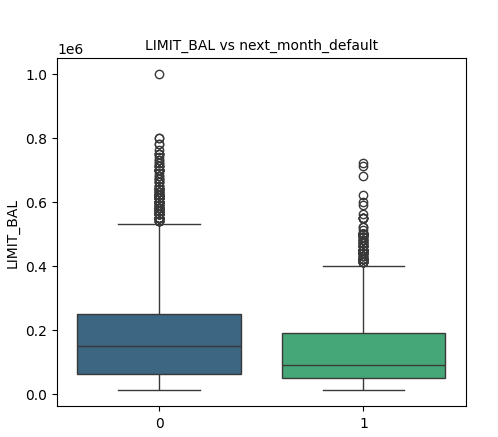
\includegraphics[width=\textwidth]{figures/1a.png}
        \caption{}
    \end{subfigure}
    \hfill
    \begin{subfigure}[b]{0.48\textwidth}
        \centering
        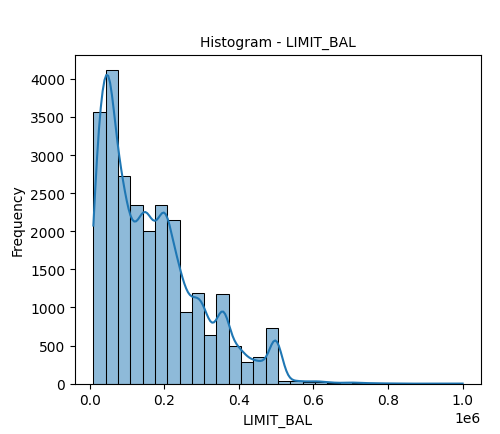
\includegraphics[width=\textwidth]{figures/1b.png}
        \caption{}
    \end{subfigure}
    \caption{(a) Boxplot of \texttt{LIMIT\_BAL} \quad (b) Histogram of \texttt{LIMIT\_BAL}}
\end{figure}

\begin{figure}[H]
    \centering
    \begin{subfigure}[b]{0.32\textwidth}
        \centering
        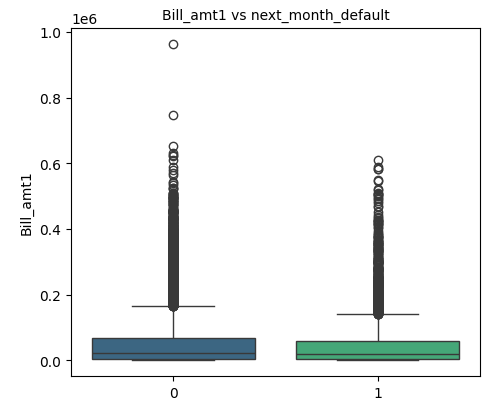
\includegraphics[width=\linewidth]{figures/2a.png}
        \caption{Boxplot of \texttt{Bill\_amt1}}
        \label{fig:univar_a}
    \end{subfigure}\hfill
    \begin{subfigure}[b]{0.32\textwidth}
        \centering
        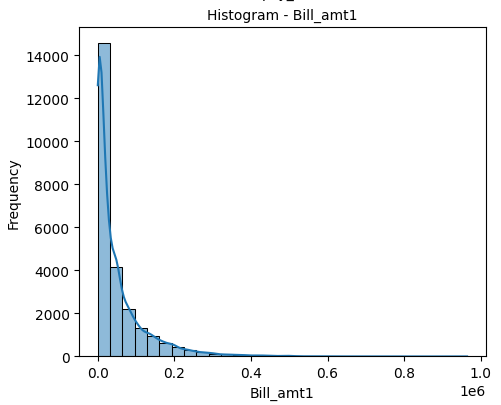
\includegraphics[width=\linewidth]{figures/2b.png}
        \caption{Histogram of \texttt{Bill\_amt1}}
        \label{fig:univar_b}
    \end{subfigure}\hfill
    \begin{subfigure}[b]{0.32\textwidth}
        \centering
        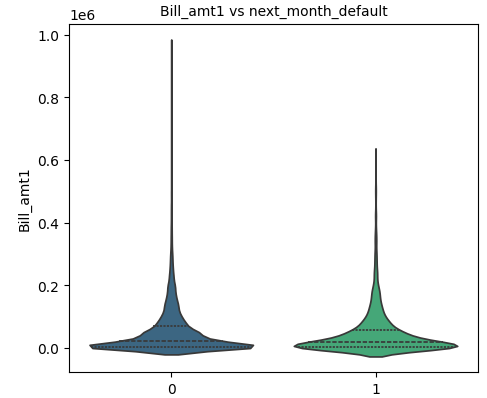
\includegraphics[width=\linewidth]{figures/2c.png}
        \caption{Violin plots of \texttt{Bill\_amt1}}
        \label{fig:univar_c}
    \end{subfigure}
    \caption{Univariate analysis: (a) \texttt{Bill\_amt1} views, (b) distributions of key features, (c) distributions stratified by default status.}
    \label{fig:univar_combined}
\end{figure}




% 2. bivariate analysis


\subsection{Bivariate Analysis}
Bivariate analysis was performed to examine the relationship between pairs of variables, primarily between independent features and the target variable \texttt{next\_month\_default}. This helps in identifying which variables are most influential in predicting defaults, and how different segments behave.
\begin{itemize}
    \item \textbf{Categorical vs Target:} Default rates varied significantly across different values of categorical variables such as \texttt{sex}, \texttt{education}, and \texttt{marriage}.
    \begin{itemize}
        \item Male customers exhibited a marginally higher default rate compared to females.
        \item Default probability was inversely related to \texttt{education} level: customers with graduate degrees had lower default rates, while those with only high school education or unspecified categories had noticeably higher default risk.
        \item Married individuals generally showed slightly lower default rates, potentially indicating more stable financial behavior.
    \end{itemize}
    \item \textbf{Monthly Payment Behavior:} Scatter plots of \texttt{pay\_amtX} vs \texttt{Bill\_amtX} revealed that defaulters often paid much less than what was billed; non-defaulters tended to pay amounts that closely matched or exceeded their billed amounts.
    \item \textbf{Payment Delay Impact:} Grouped barplots using the \texttt{pay\_0} feature showed that higher delay values are associated with increased default probability. Customers who had payment delays of 2 months or more were significantly more likely to default.
\end{itemize}
\begin{figure}[H]
    \centering
    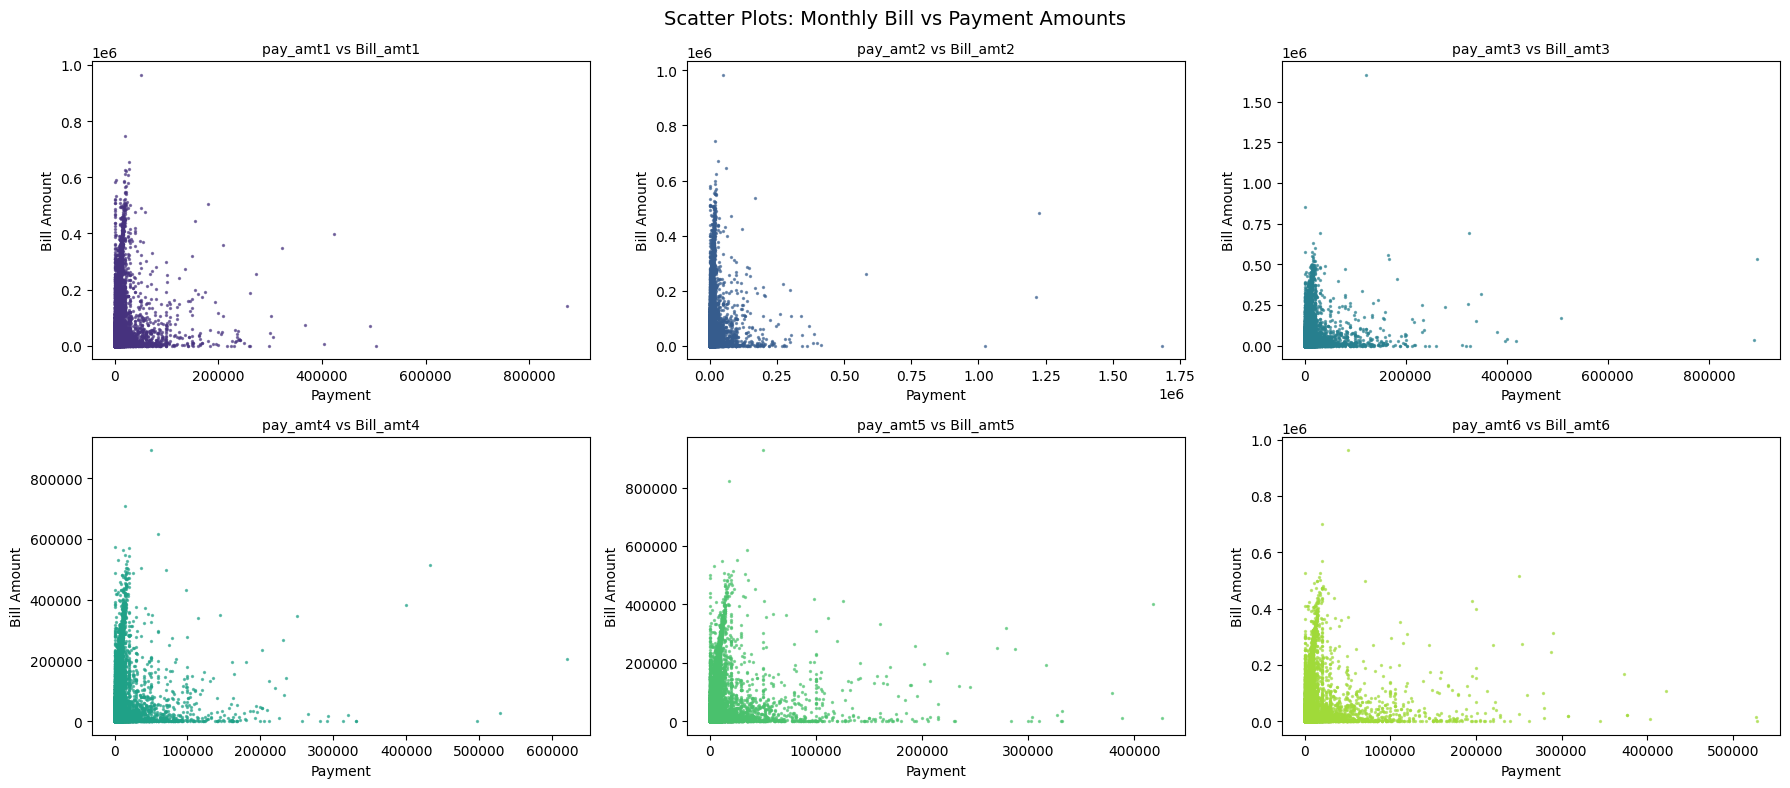
\includegraphics[width=1\textwidth]{figures/3.png}
    \caption{Scatter plot of \texttt{pay\_amtX} vs \texttt{Bill\_amtX}}
\end{figure}

% \begin{figure}[H]
%     \centering
%     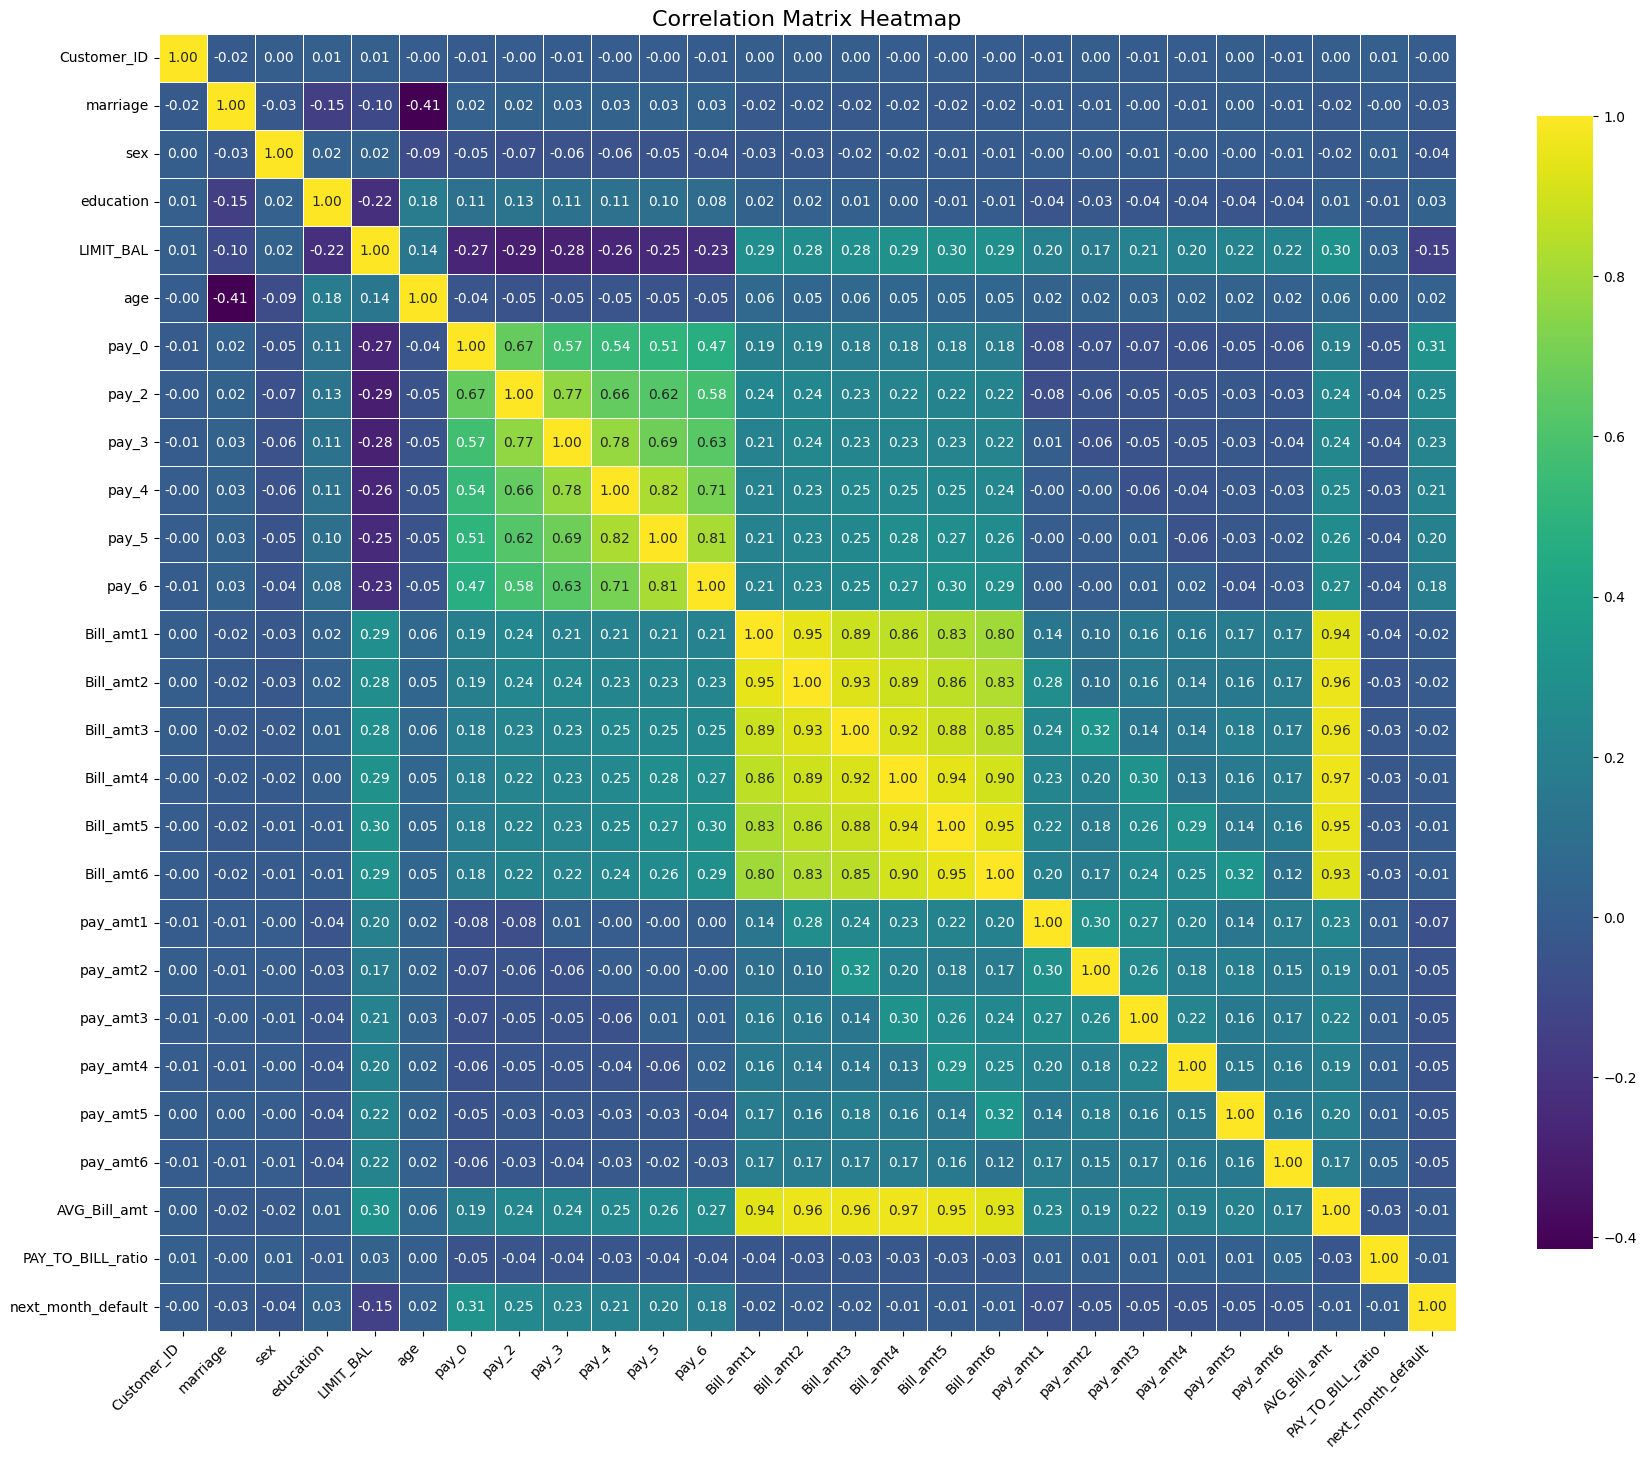
\includegraphics[width=0.8\textwidth]{figures/4.png}
%     \caption{Correlation Matrix}
% \end{figure}

\subsection{Correlation Analysis}
From the correlation heatmap we can observe:
\begin{itemize}
    \item There is a high correlation between delayed payments (\texttt{pay\_x}) and defaults, and \texttt{Bill\_amtX} and \texttt{pay\_amtX} also have high correlation.
    \item Strong positive correlations were found among consecutive billing amounts (\texttt{Bill\_amt1} to \texttt{Bill\_amt6}) and among payment amounts (\texttt{pay\_amt1} to \texttt{pay\_amt6}). This indicates temporary stability in customer billing/payment behavior but also suggests potential multicollinearity.
    \item Payment delay features (\texttt{pay\_0} to \texttt{pay\_6}) were moderately correlated with each other, and \texttt{pay\_1} showed the strongest linear correlation with the target variable \texttt{next\_month\_default} (0.31).
    \item Features like \texttt{LIMIT\_BAL}, \texttt{age}, and demographic attributes had relatively low correlation with default.
    \item Based on correlation thresholding (e.g., removing one of any pair with $|\rho| > 0.9$), redundant features were dropped to reduce noise and improve model generalization.
\end{itemize}
\begin{figure}[H]
    \centering
    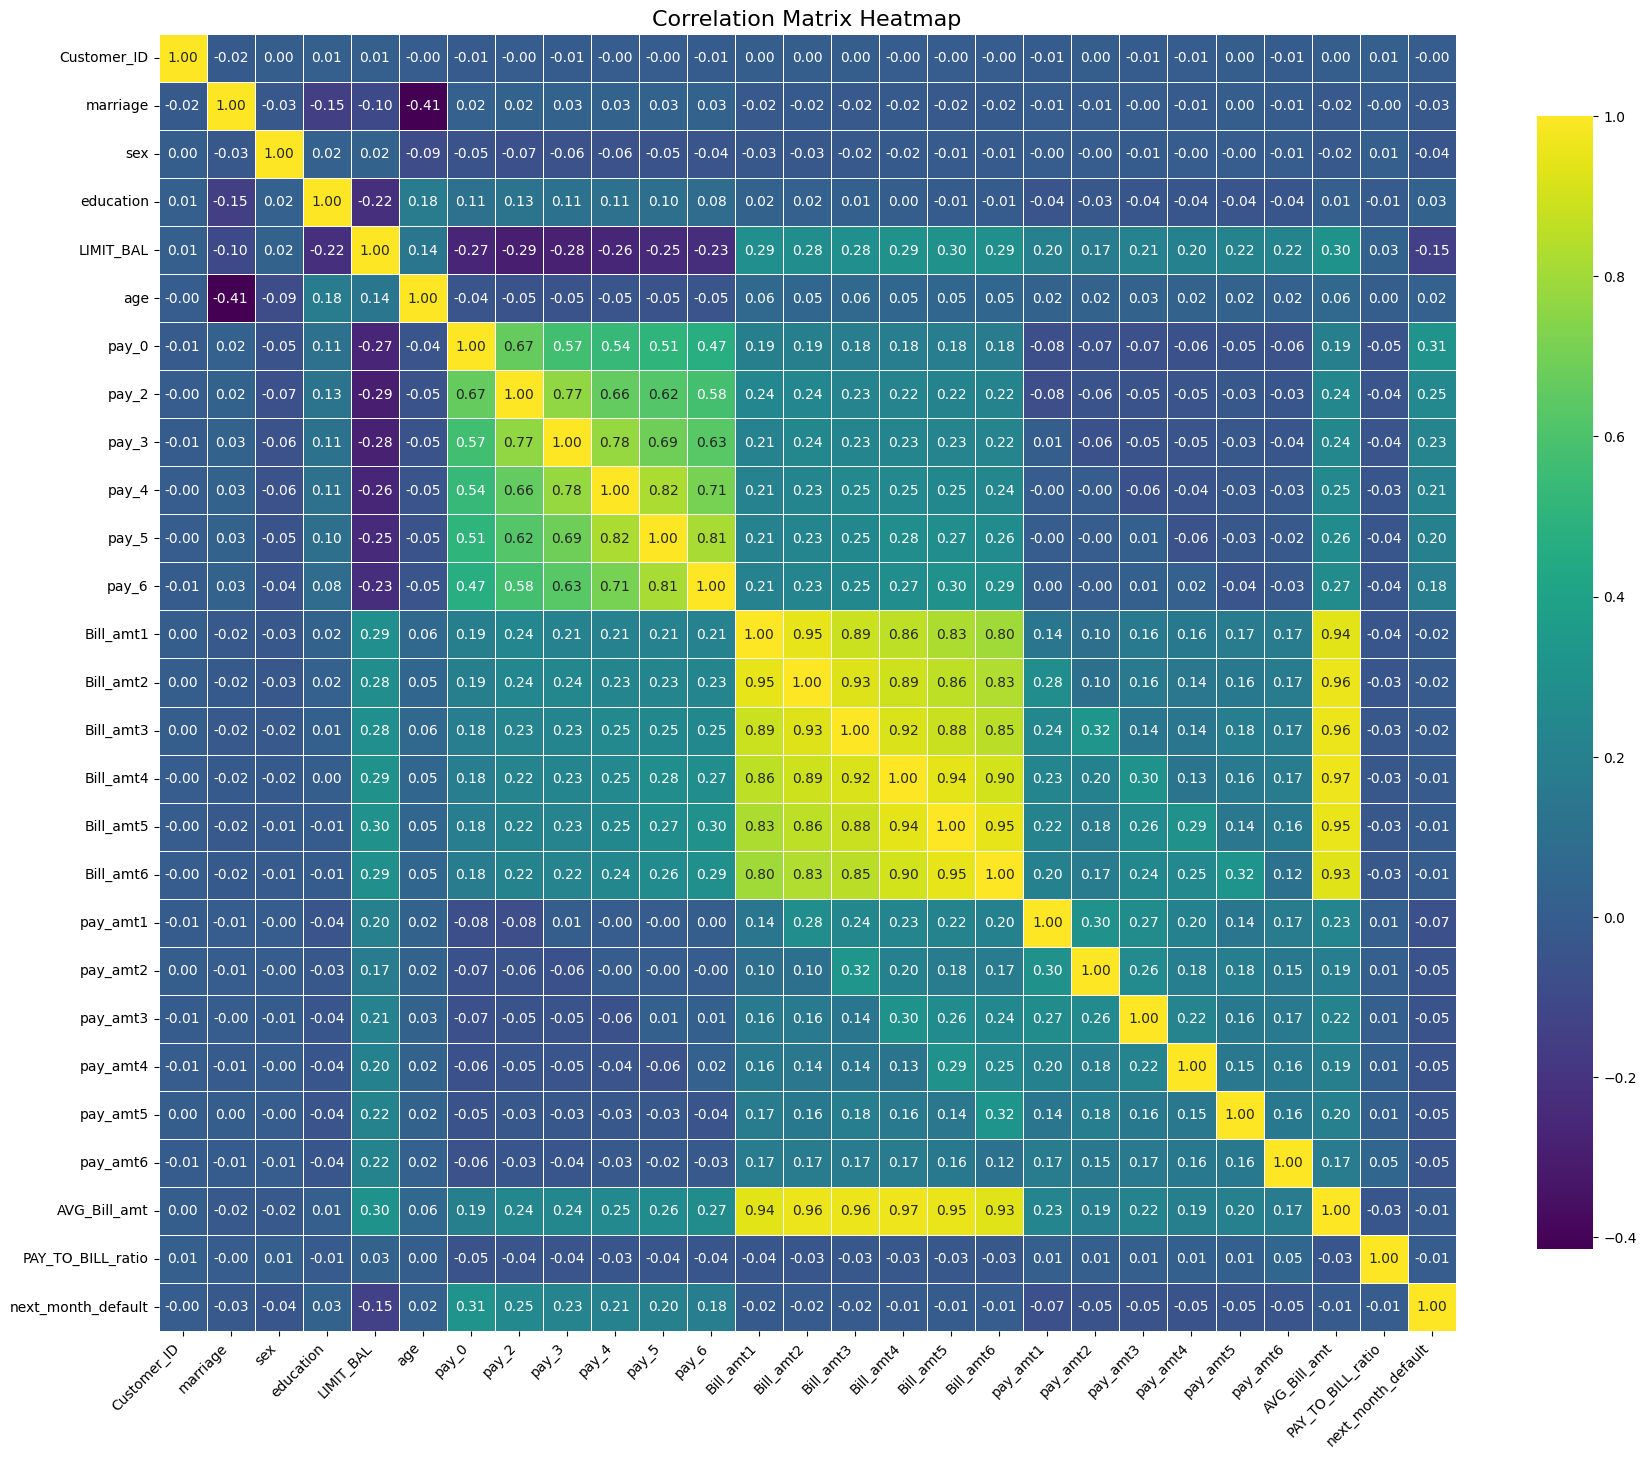
\includegraphics[width=1\textwidth]{figures/4.png}
    \caption{Correlation Matrix}
\end{figure}

\subsection{Bill and Payment Amount Patterns}
\begin{itemize}
    \item Bill Amounts: Although the absolute bill amount was not a strong predictor, defaulters tended to have more volatile monthly bills.
    \item Payment Amounts: Defaulters showed lower consistency in payment behavior, often underpaying compared to the billed amount.
    \item Repayment Ratios: Many defaulters had low \texttt{PAY\_TO\_BILL} ratio values, indicating insufficient or delayed repayment.
\end{itemize}
\begin{figure}[H]
    \centering
    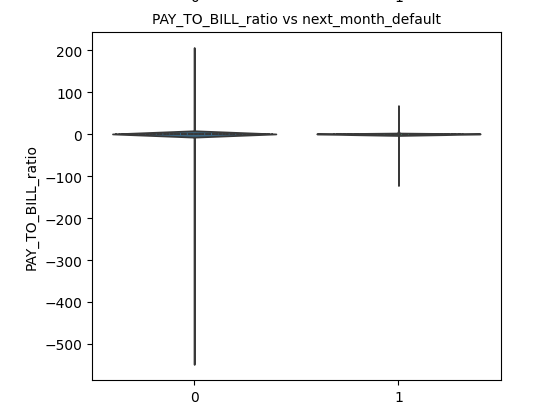
\includegraphics[width=0.6\textwidth]{figures/5.png}
    \caption{Violin plot of \texttt{PAY\_TO\_BILL} ratio by default status}
\end{figure}

\subsection{Demographic Variables}
\begin{itemize}
    \item \texttt{sex}: Male customers default rate is visibly higher than female.
    \item \texttt{education}: Customers with lower education levels (especially category 3 = High School or below) were more likely to default than customers with graduation or university education level, indicating a possible link between financial literacy and credit behavior.
    \item \texttt{marriage}: No strong trend emerged across marital categories, but single customers had marginally higher default risk.
    \item \texttt{age}: Younger customers (aged 21--30) exhibited the highest default rates. Older customers (above 45) showed more conservative credit behavior.
\end{itemize}
\begin{figure}[H]
    \centering
    \begin{subfigure}{0.8\textwidth}
        \centering
        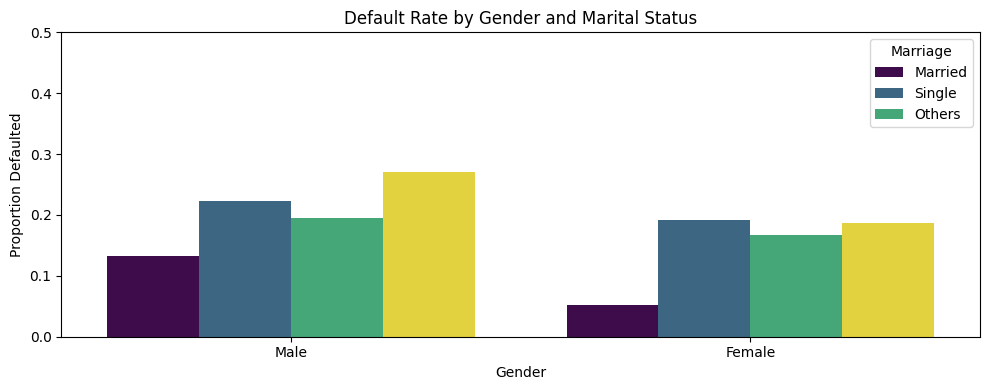
\includegraphics[width=\textwidth]{figures/6a.png}
        \caption{Default rate by age groups}
    \end{subfigure}
    
    \vspace{0.6em}
    \begin{subfigure}{0.8\textwidth}
        \centering
        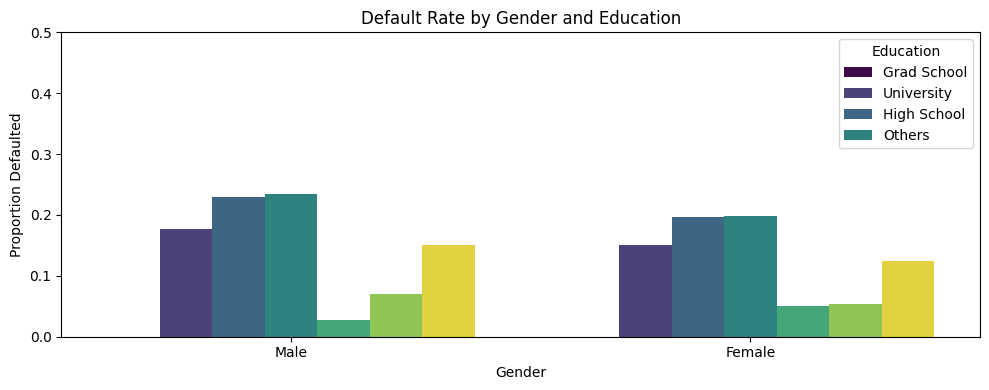
\includegraphics[width=\textwidth]{figures/6b.png}
        \caption{Default rate comparison across \texttt{sex}, \texttt{age}, \texttt{education}, and \texttt{marriage}}
    \end{subfigure}
    
    \vspace{0.6em}
    \begin{subfigure}{0.8\textwidth}
        \centering
        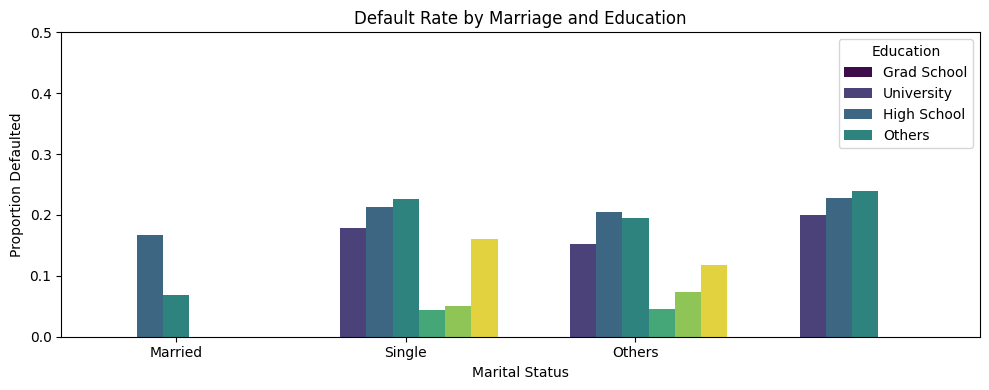
\includegraphics[width=\textwidth]{figures/6c.png}
        \caption{Demographic analysis by gender, education and marriage status}
    \end{subfigure}
    
    \caption{Demographic variable influence on default behaviour}
    \label{fig:demographic_vertical}
\end{figure}

\subsection{Repayment Status (\texttt{pay\_0} to \texttt{pay\_6})}
The repayment status variables had the strongest relationship with default:
\begin{itemize}
    \item Defaulters consistently had higher values in \texttt{pay\_x} variables (indicating delays).
    \item A trend of increasing delay over consecutive months was observed among defaulters.
    \item Non-defaulters mostly had \texttt{pay\_x} values of \texttt{-1} (fully paid on time) or \texttt{0} (partial but non-delinquent).
\end{itemize}



% next : complete section 3

\section{Data Preprocessing}
A comprehensive data preprocessing pipeline was applied prior to modeling. This included handling categorical variables, transforming numerical features, and preparing the dataset for balanced training.

\subsection{Handling Missing Values}
The dataset had 126 missing values in the \texttt{age} column. From EDA we can see that the distribution curve is highly skewed. So, using the \texttt{median} strategy of \texttt{SimpleImputer} was best for filling in missing values of the \texttt{age} column.
\begin{figure}[H]
    \centering
    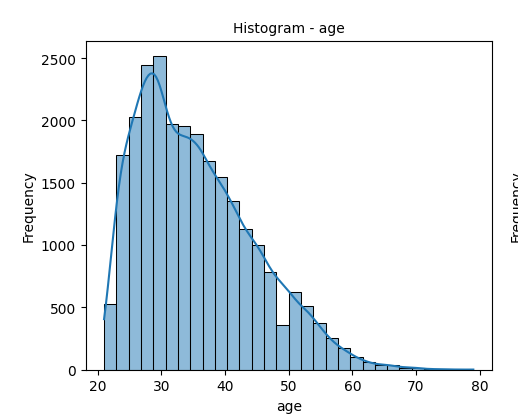
\includegraphics[width=0.6\textwidth]{figures/7.png}
    \caption{Distribution of \texttt{age}}
\end{figure}

\subsection{Normalization of Categorical Features}
We observed that some categorical variables such as \texttt{education} and \texttt{marriage} contained undefined values.
\begin{itemize}
    \item \texttt{education}: Valid categories included 1 = Graduate School, 2 = University, 3 = High School, and 4 = Others. Values beyond this range (such as 5, 6 and 0) were recoded as 4 (Others) to preserve the data.
    \item \texttt{marriage}: Values like 1 = Married, 2 = Single, and 3 = Others were valid. Unexpected values like 0 were reassigned to 3 (Others).
\end{itemize}
\begin{figure}[H]
    \centering
    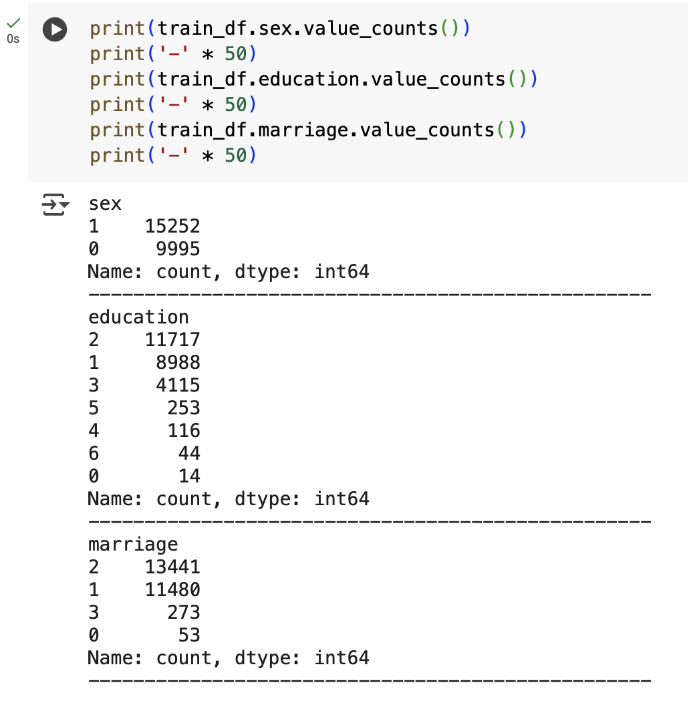
\includegraphics[width=0.6\textwidth]{figures/8.png}
    \caption{Value Count of Categorical Variables}
\end{figure}

\subsection{Correlation Filtering}
Highly correlated features: \texttt{Bill\_amt1}, \texttt{Bill\_amt2}, \texttt{Bill\_amt3}, \texttt{Bill\_amt4}, \texttt{Bill\_amt5}, \texttt{pay\_amt2}, \texttt{pay\_amt3}, \texttt{pay\_amt4}, \texttt{pay\_amt5}, \texttt{pay\_amt6} were dropped to reduce multicollinearity and avoid overfitting without significant information loss.
\begin{figure}[H]
    \centering
    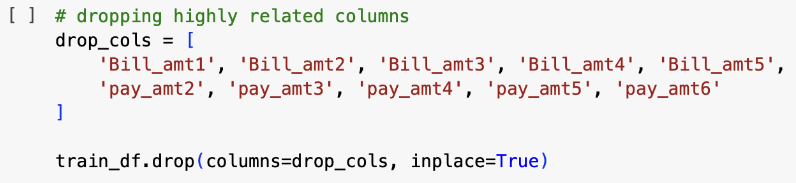
\includegraphics[width=0.6\textwidth]{figures/9.png}
    \caption{Correlation filtering code snippet}
\end{figure}

\subsection{Encoding}
We encoded categorical variables by using OneHot Encoding. This was necessary to convert categorical variables into a set of binary (0/1) columns because the ML algorithms we are going to use cannot handle strings or categories directly. They expect numerical input.

\subsection{Scaling, Splitting, and Balancing with SMOTE}
To prepare the data for model training, we applied:
\begin{itemize}
    \item \textbf{Train-Test Split:} The dataset was split into training and test sets in an 80:20 ratio using stratified sampling to preserve the proportion of default vs. non-default classes across both sets.
    \item \textbf{Standardization:} All numerical features were standardized using \texttt{StandardScaler}, transforming to have 0 mean and unit variance.
    \item \textbf{SMOTE:} As the target variable \texttt{next\_month\_default} was highly imbalanced, with fewer defaulters than non-defaulters, we applied \texttt{SMOTE} to the training set. SMOTE helps improve recall and ensures the classifier is not biased toward the majority class.
    \item It is necessary to note here that train-test split must be performed before SMOTE. Because if we apply SMOTE before splitting, information from your test set leaks into your training set. This is called data leakage and can lead to overly optimistic model performance — our model learns patterns that it shouldn't know yet.
\end{itemize}
\begin{figure}[H]
    \centering
    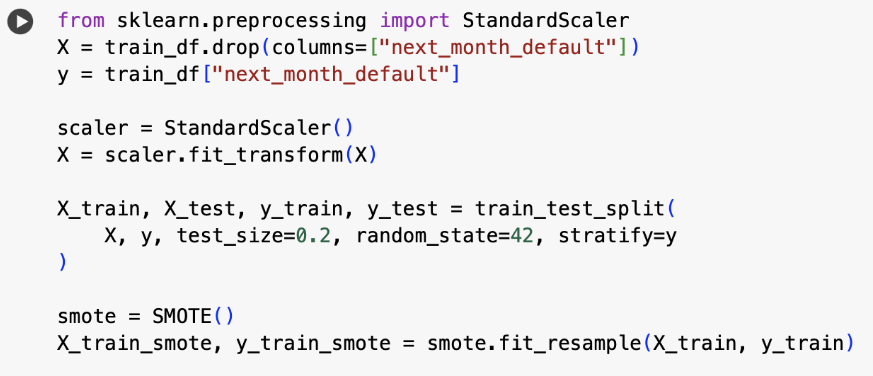
\includegraphics[width=0.6\textwidth]{figures/10.png}
    \caption{SMOTE code snippet}
\end{figure}

Visualizing Class Balance: The bar plots in Figure~\ref{fig:smote_class_balance} show the class distribution before and after applying SMOTE. The left plot confirms the class imbalance in the original training data, while the right plot shows balanced classes after resampling.
\begin{figure}[H]
    \centering
    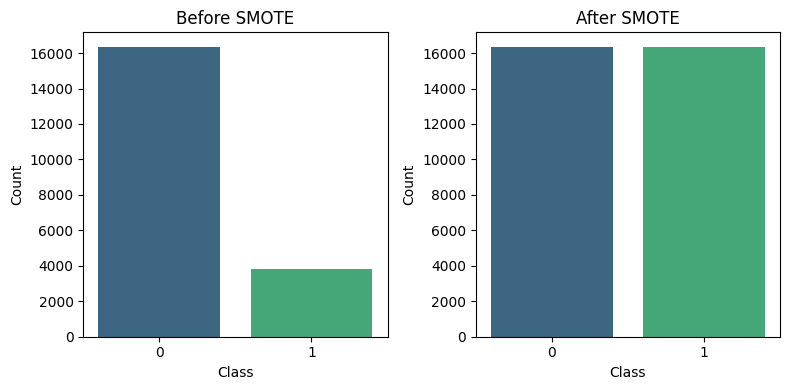
\includegraphics[width=0.8\textwidth]{figures/11.png}
    \caption{Class Distribution Before and After SMOTE}
    \label{fig:smote_class_balance}
\end{figure}

Quantitative Comparison: A summary of the number of samples in each class before and after SMOTE is shown below:
\begin{table}[H]
    \centering
    \begin{tabular}{lcc}
        \toprule
        Class & Before SMOTE & After SMOTE \\
        \midrule
        No Default (0) & 16352 & 16352 \\
        Default (1) & 3845 & 16352 \\
        \bottomrule
    \end{tabular}
    \caption{Class Counts Before and After SMOTE Resampling}
\end{table}


% next 

\section{Financial Feature Engineering}

To enhance model performance and improve interpretability, we engineered a set of financial features
that capture customer behavior patterns more effectively than the raw variables alone. These
derived features were created based on domain knowledge of credit risk, with a focus on repayment
consistency, utilization, volatility, and delinquency.

\begin{itemize}
    \item \textbf{avg utilization ratio}: Measures the average proportion of the credit limit used by the customer over six months. High values indicate aggressive credit use, which correlates with higher default risk.
    \item \textbf{underpay ratio}: Captures the tendency of a customer to consistently pay less than their billed amount. It is computed as the proportion of months where payment was significantly lower than the bill.
    \item \textbf{zero payment months}: Counts the number of months where no payment was made despite having an outstanding bill. This helps flag chronic non-payers.
    \item \textbf{repayment consistency}: Calculates the standard deviation of the \texttt{pay\_x} values over six months. Higher values suggest erratic repayment behavior.
    \item \textbf{bill volatility} and \textbf{payment std}: Measure fluctuations in bill amounts and payment amounts respectively. High volatility often implies poor financial planning or unstable cash flow.
    \item \textbf{max delay} and \textbf{avg delay value}: Represent the longest and average payment delay (in months) experienced by the customer. These are direct indicators of repayment discipline.
    \item \textbf{delinquency streak}: Flags customers who had consecutive months of overdue payments, reflecting prolonged financial stress.
    \item \textbf{avg payment ratio}: Represents the ratio of actual payment to billed amount, averaged over six months. Low values are indicative of habitual underpayment.
    \item \textbf{total underpaid amount} and \textbf{total overpaid amount}: Capture cumulative payment deviations from expected amounts, helping the model understand payment surplus or deficit patterns.
    \item \textbf{monthly payment range}, \textbf{avg payment amount}, and \textbf{avg bill amount}: Summarize the range and average of billing/payment behavior to enhance model stability across varying customer profiles.
\end{itemize}

\section{Modeling Strategy}

We trained many models like Logistic Regression, Decision Tree, Random Forest, XGBoost,
LightGBM. This section provides a detailed walkthrough of each modeling phase including model
training, hyperparameter tuning, threshold optimization, ensemble learning, and final evaluation.

\subsection{Model Training}

These are the metrics obtained fro each model trained:

\begin{figure}[H]
    \centering
    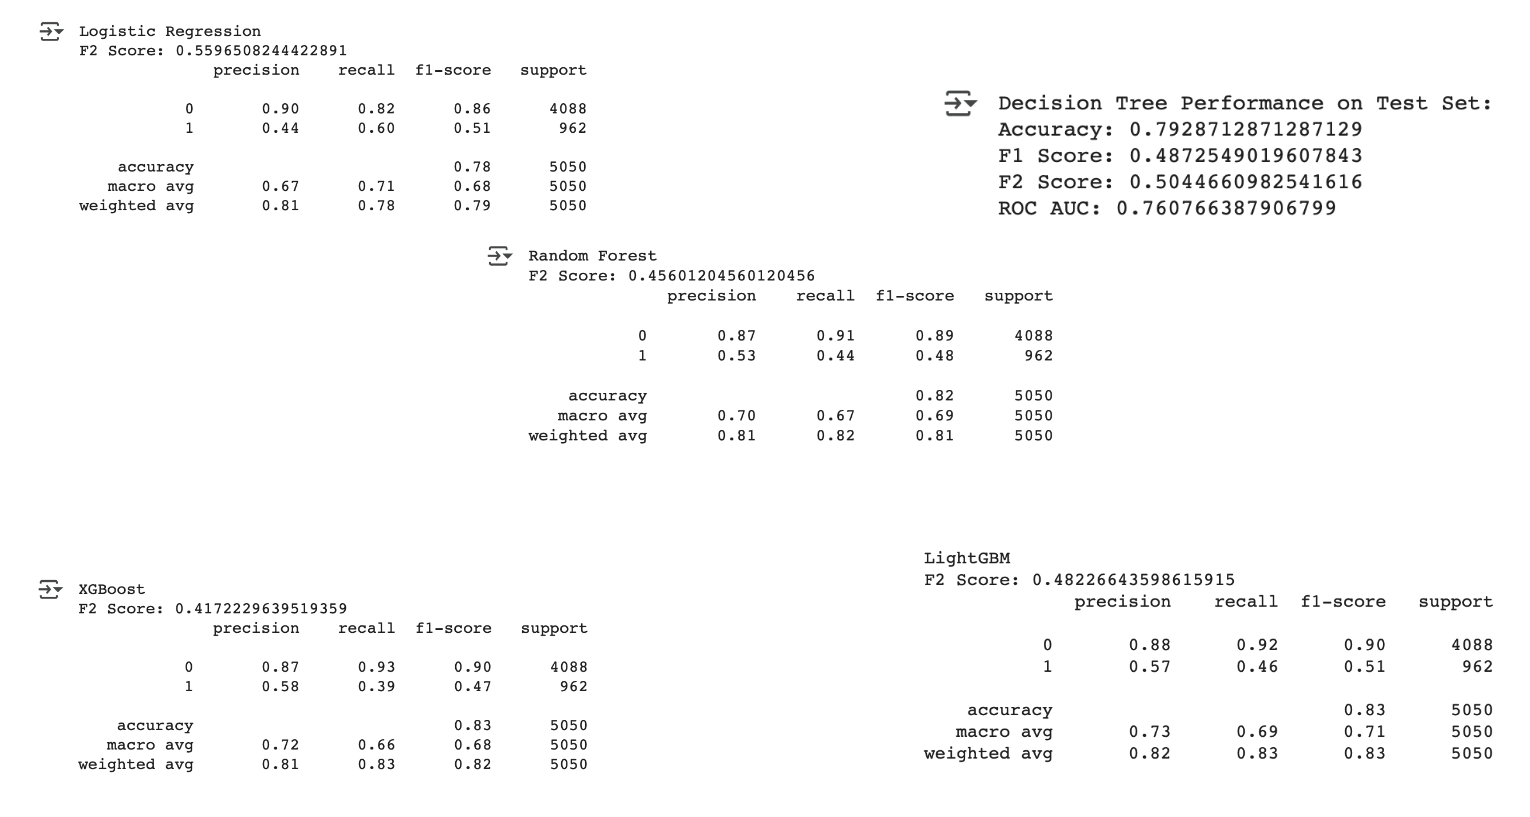
\includegraphics[width=1\textwidth]{figures/14a.png}
\end{figure}
\begin{figure}[H]
    \centering
    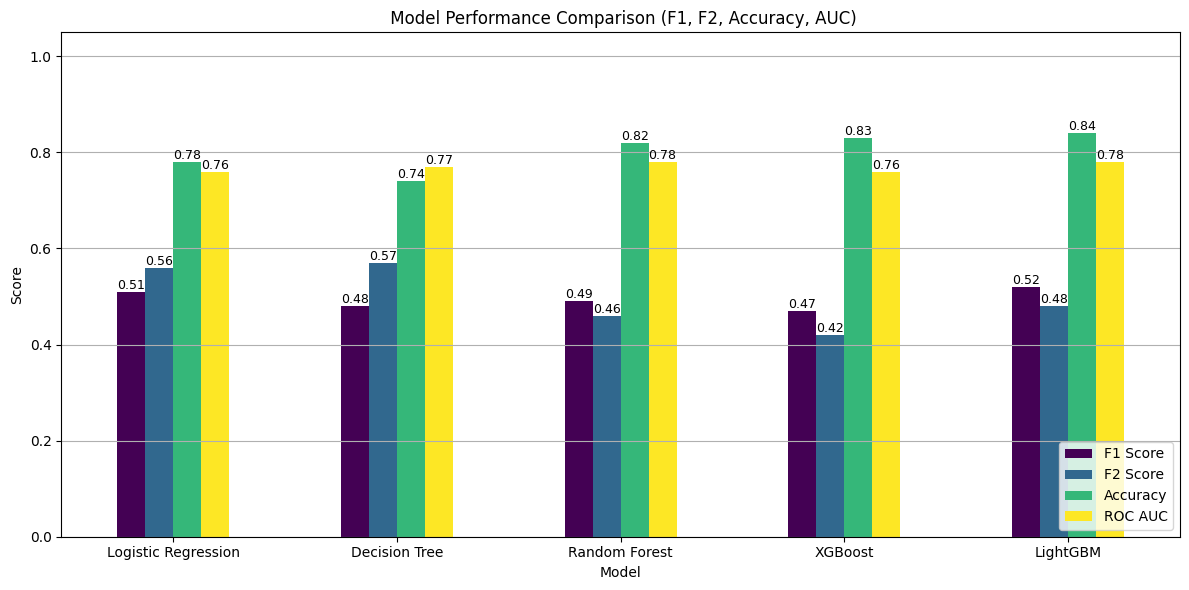
\includegraphics[width=1\textwidth]{figures/14b.png}
    \caption{Comparision Bar chart of baseline models trained}
\end{figure}



\subsection{Threshold Optimization}

Rather than relying on the default 0.5 threshold, we swept thresholds from 0.1 to 0.9 and evaluated
each using F1, F2, and Accuracy. Table \ref{tab:thresholds_f2} shows the thresholds that gave the best F2-score for each
model.

\begin{table}[H]
\centering
\caption{Thresholds Optimized for F2-Score}
\label{tab:thresholds_f2}
\begin{tabular}{lccccc}
\toprule
Model & Threshold & F1 Score & F2 Score & Accuracy & ROC AUC \\
\midrule
Logistic Regression & 0.37 & 0.417 & 0.508 & 0.579 & 0.761 \\
Random Forest & 0.38 & 0.47 & 0.60 & 0.69 & 0.78 \\
XGBoost & 0.30 & 0.48 & 0.53 & 0.77 & 0.76 \\
LightGBM & 0.30 & 0.50 & 0.57 & 0.78 & 0.78 \\
\bottomrule
\end{tabular}
\end{table}

We did not used Threshold Optimization on Decision Tree because our F2 Score is stuck at 0.412
across all thresholds, It suggests that model isn't capturing minority class singnals well, despite
SMOTE and \texttt{class\_weight='balanced'}.
So we use Grid Search CV for hyperparameter tuning of decision tree.

\begin{figure}[H]
    \centering
    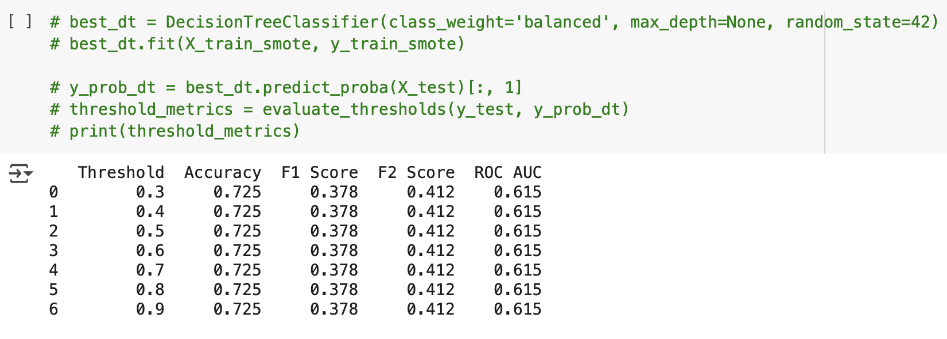
\includegraphics[width=0.8\textwidth]{figures/15.png}
    \caption{Thresholds of Decision Tree}
\end{figure}

\begin{figure}[H]
    \centering
    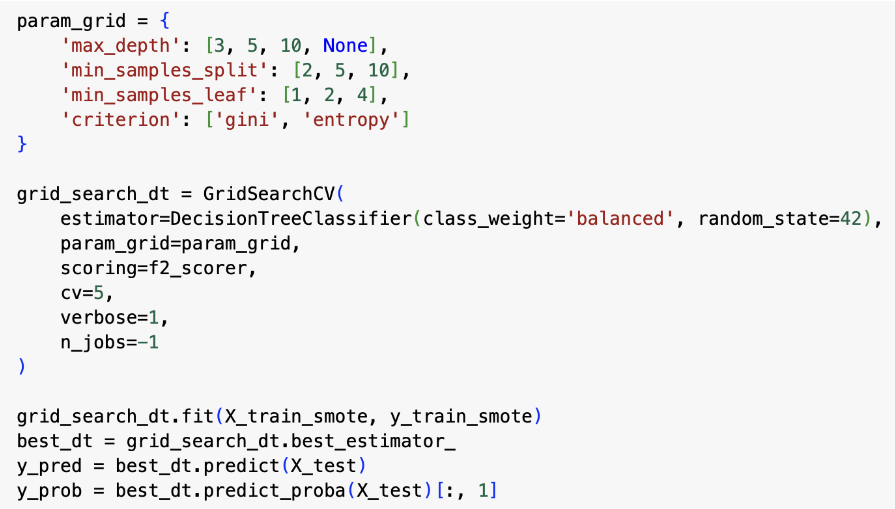
\includegraphics[width=0.8\textwidth]{figures/16.png}
    \caption{Code Snippet for GridSearchCV}
\end{figure}

\begin{figure}[H]
    \centering
    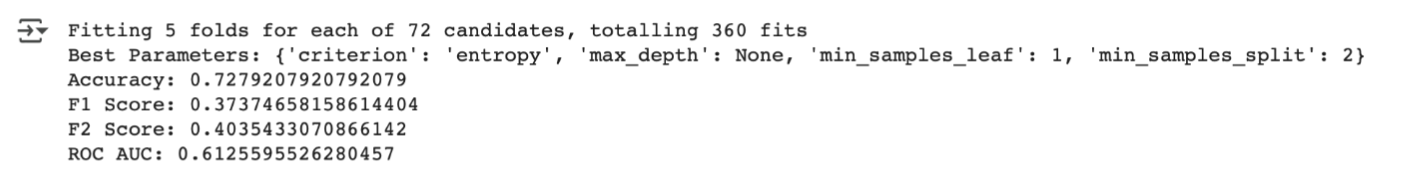
\includegraphics[width=0.7\textwidth]{figures/17.png}
    \caption{Decision Tree evaluation metrics after grid search cv}
\end{figure}

\subsection{Ensemble Learning}

To further improve predictive performance, we constructed ensemble models:
\begin{itemize}
    \item \textbf{Stacking Classifier:} Combined predictions from the top four base learners (LogReg, DT,
    LightGBM), with a logistic regression meta-model. This model achieved the best F2-score
    i.e. 0.60 on the test set after threshold tuning but low accuracy of 0.57.
    \item \textbf{Voting Classifier:} A soft-voting ensemble averaged the predicted probabilities. It performed comparably but slightly worse than stacking in F2-score.
\end{itemize}

\subsection{Final Evaluation}

Table \ref{tab:final_eval} summarizes the test-set performance.

\begin{table}[H]
\centering
\caption{Final Model Evaluation Metrics on Test Set}
\label{tab:final_eval}
\begin{tabular}{lcccc}
\toprule
Model & F1 Score & F2 Score & Accuracy & ROC AUC \\
\midrule
Stacked Ensemble & 0.42 & 0.60 & 0.58 & 0.78 \\
Voting Classifier & 0.52 & 0.48 & 0.83 & 0.79 \\
Tuned Logistic Regression & 0.42 & 0.58 & 0.58 & 0.76 \\
Tuned Decision Tree & 0.37 & 0.40 & 0.73 & 0.61 \\
Tuned Random Forest & 0.47 & 0.60 & 0.69 & 0.78 \\
Tuned XGBoost & 0.48 & 0.53 & 0.77 & 0.76 \\
Tuned LightGBM & 0.51 & 0.57 & 0.78 & 0.78 \\
\bottomrule
\end{tabular}
\end{table}


\begin{figure}[H]
    \centering
    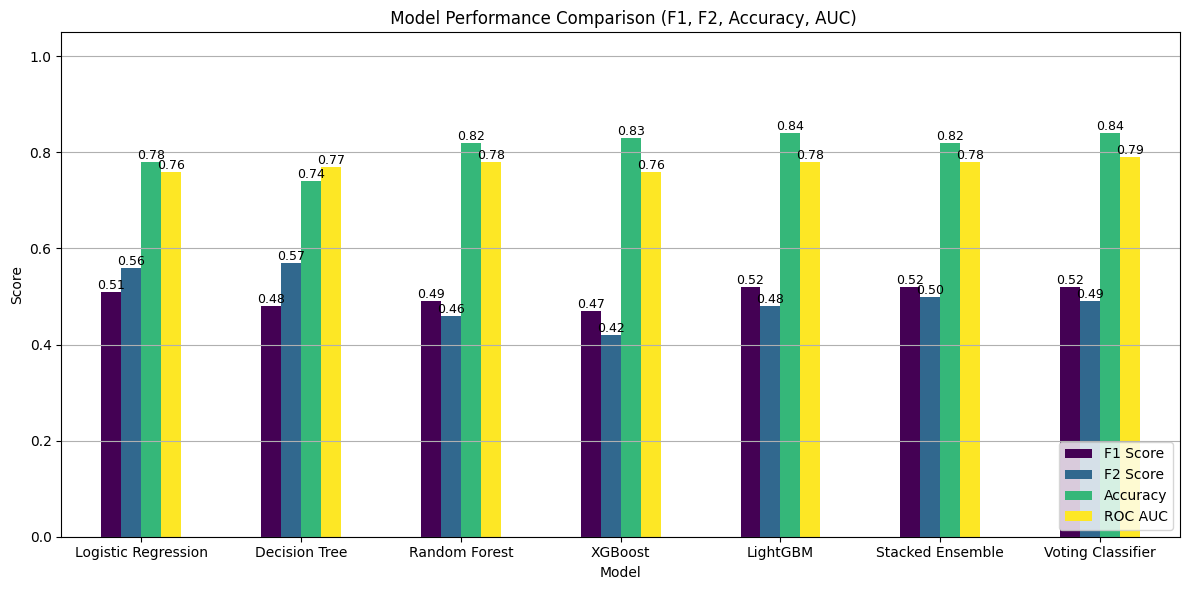
\includegraphics[width=1\textwidth]{figures/18.png}
    \caption{Comparision Chart Tuned Models}
\end{figure}



% \begin{figure}[H]
%     \centering
%     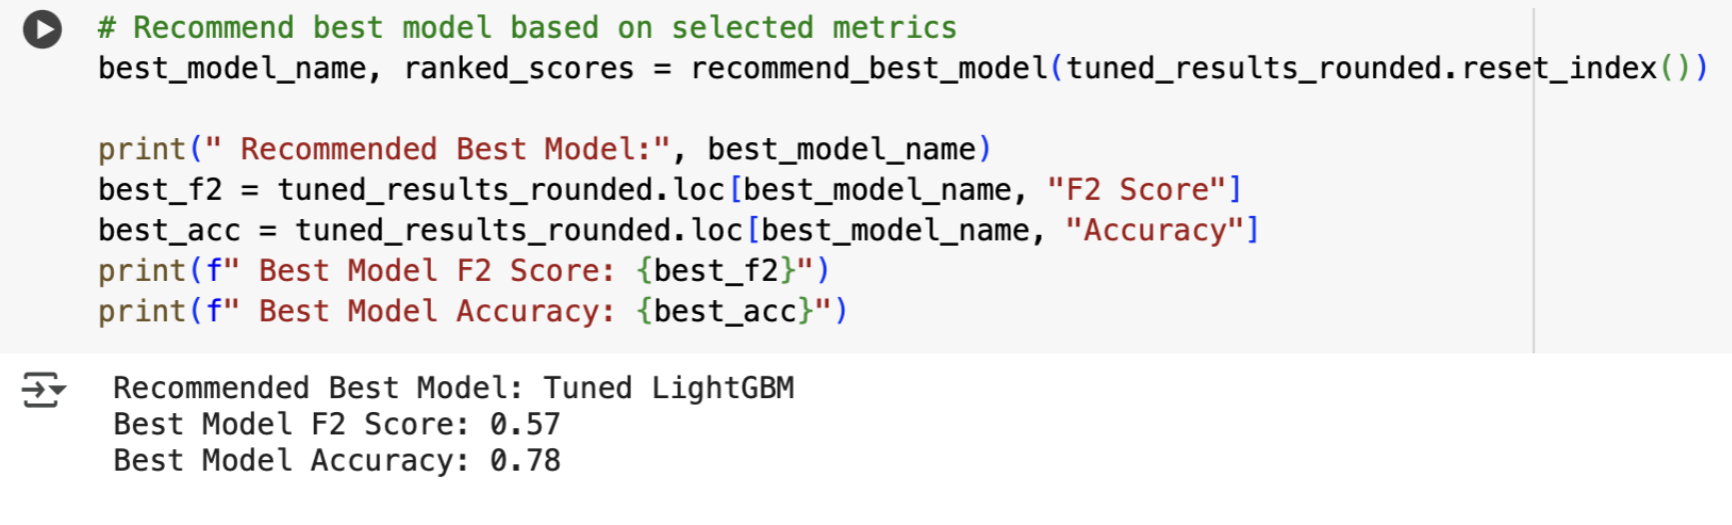
\includegraphics[width=0.8\textwidth]{figures/19.png}
%     \caption{Best Model Code snippet}
% \end{figure}

In the context of credit risk prediction, minimizing false negatives is more critical than minimizing
false positives. A false negative corresponds to a risky customer who is predicted as non-defaulter,
potentially resulting in financial loss to the credit institution.

To reflect this business priority, we chose the F2-score as our primary evaluation metric. F2-
score places more emphasis on recall. This aligns with our goal of maximizing the detection of
potential defaulters.

Therefore, all model selection, hyperparameter tuning, and threshold optimization steps were
guided by the goal of maximizing F2-score while maintaining reasonable values for accuracy and
F1-score.
The final recommended model we got was Tuned LightGBM, having nice F2 score along with
Accuracy.

\begin{figure}[H]
    \centering
    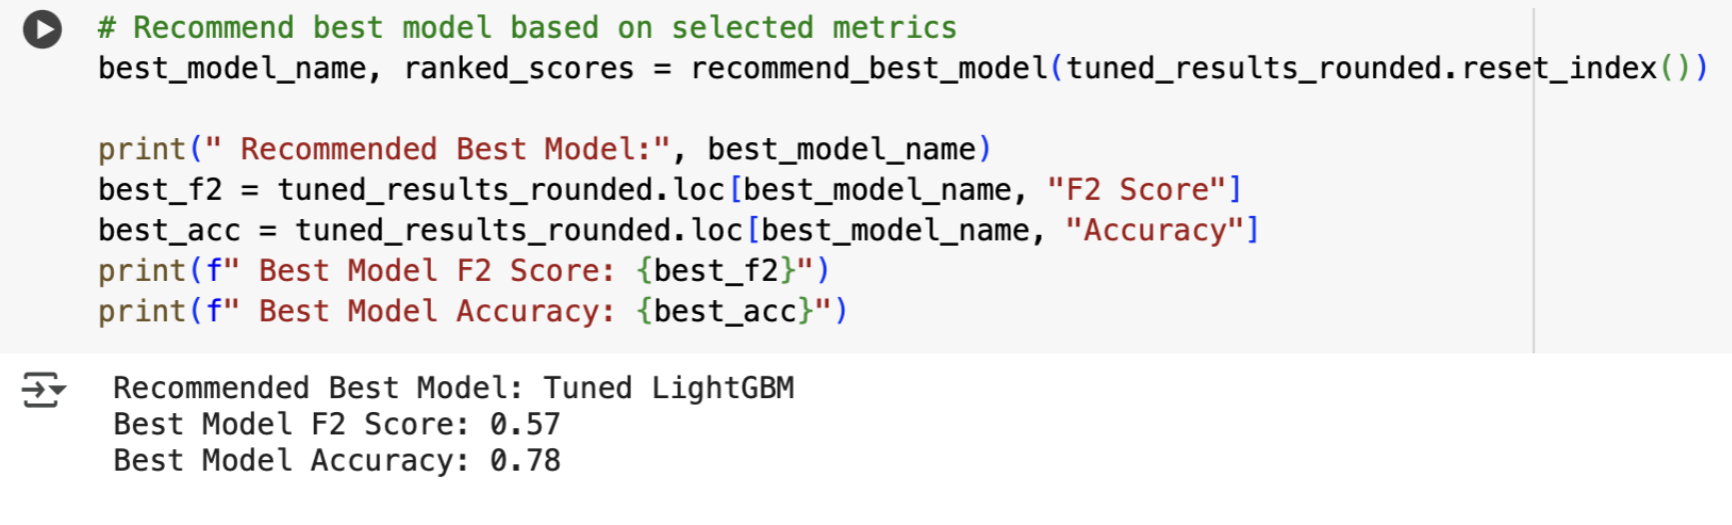
\includegraphics[width=0.8\textwidth]{figures/19.png}
    \caption{Best Model Code snippet}
\end{figure}


\begin{figure}[H]
    \centering
    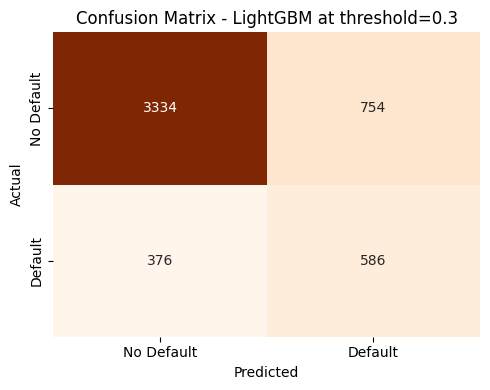
\includegraphics[width=0.5\textwidth]{figures/20.png}
    \caption{Best Model Report}
\end{figure}

% \begin{figure}[H]
%     \centering
%     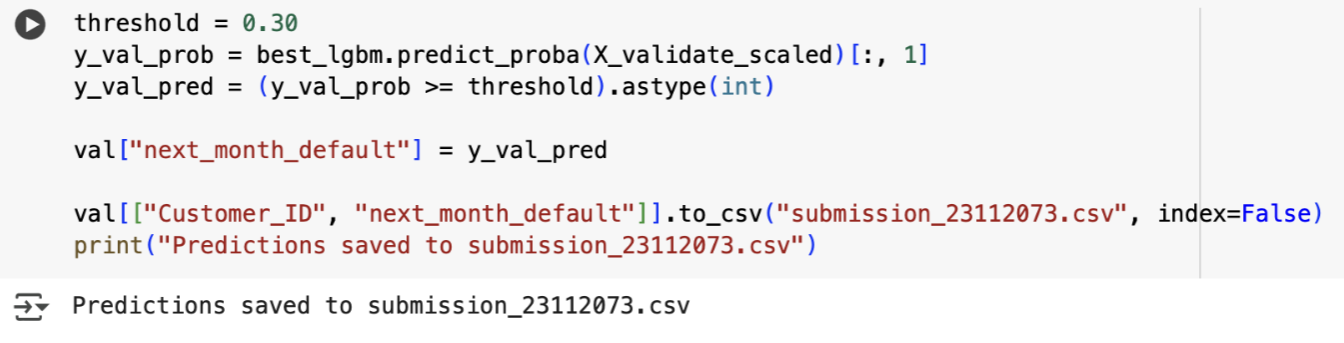
\includegraphics[width=0.8\textwidth]{figures/21.png}
%     \caption{Best Model Report}
% \end{figure}




% last part 


\section{Validation Predictions}

On the unlabeled validation dataset, predictions were generated using the final tuned model and stored in a CSV format with two columns: \texttt{Customer}, \texttt{next\_month\_default}. The Best Model was applied to the unlabeled validation dataset after applying the same preprocessing and threshold.

\begin{figure}[H]
    \centering
    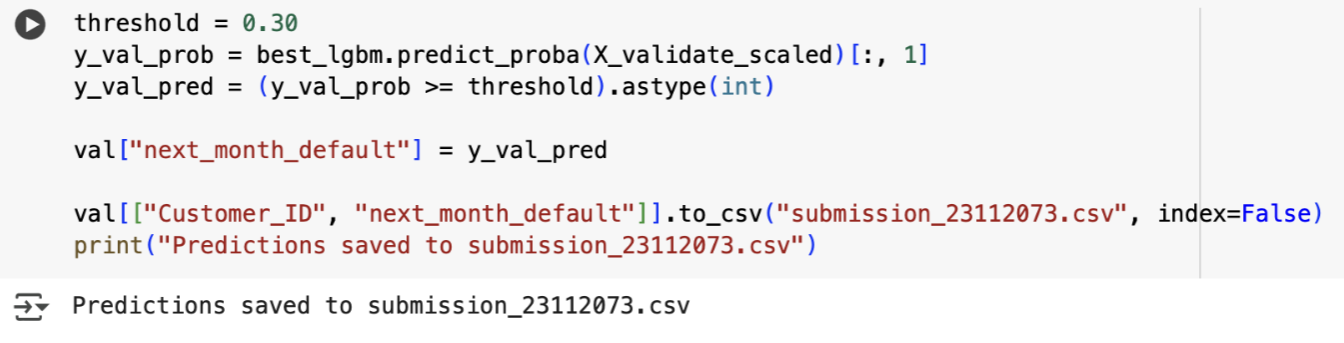
\includegraphics[width=0.8\textwidth]{figures/21.png}
    \caption{Validation Code}
\end{figure}

\section{Selection of F2-Score Over Other Metrics}

Several evaluation metrics were considered during model development, including Accuracy, Precision, Recall, F1-score, F2-score, and ROC-AUC. However, after reviewing the business context and implications of misclassification, the F2-score was prioritized as the primary model selection criterion.

\begin{itemize}
    \item \textbf{Accuracy}: due to class imbalance a model could achieve high accuracy by simply predicting the majority class (non-defaulters), while missing most actual defaulters.
    \item \textbf{Precision} measures how many predicted defaulters were truly defaulters. But precision alone does not penalize the model for missing actual defaulters, which is costlier in credit risk applications.
    \item \textbf{Recall} emphasizes capturing all actual defaulters, which is more aligned with our goal. However, recall alone ignores how many false positives the model generates.
    \item \textbf{F1-score} balances precision and recall equally, but in our domain, recall is more valuable. Missing a defaulter (false negative) is riskier than flagging a safe customer (false positive).
    \item \textbf{F2-score}, which weights recall more heavily than precision, was therefore selected. It ensures that the model is more sensitive to defaulters, reducing the chance of financial exposure due to missed risks.
    \item \textbf{ROC-AUC} was used as a supporting metric to evaluate the model's overall prediction ability, but F2-score guided actual classification threshold tuning and model choice.
\end{itemize}

Ultimately, F2-score was the most suitable metric. All model tuning and threshold optimization were conducted with the objective of maximizing F2-score while maintaining acceptable levels of F1-score and accuracy.

\section{Conclusion}

This model predicted 27.01\% as defaulters which is greater than the actual defaulters (19.04\%) train dataset had (real world). This model provides a risk-sensitive, interpretable scoring system that supports Bank A's early-warning strategy. By combining robust EDA, financial engineering, and tuned classification pipelines, the solution aligns technical accuracy with business impact.




\end{document}

